% Options for packages loaded elsewhere
\PassOptionsToPackage{unicode}{hyperref}
\PassOptionsToPackage{hyphens}{url}
%
\documentclass[
]{article}
\usepackage{lmodern}
\usepackage{amssymb,amsmath}
\usepackage{ifxetex,ifluatex}
\ifnum 0\ifxetex 1\fi\ifluatex 1\fi=0 % if pdftex
  \usepackage[T1]{fontenc}
  \usepackage[utf8]{inputenc}
  \usepackage{textcomp} % provide euro and other symbols
\else % if luatex or xetex
  \usepackage{unicode-math}
  \defaultfontfeatures{Scale=MatchLowercase}
  \defaultfontfeatures[\rmfamily]{Ligatures=TeX,Scale=1}
\fi
% Use upquote if available, for straight quotes in verbatim environments
\IfFileExists{upquote.sty}{\usepackage{upquote}}{}
\IfFileExists{microtype.sty}{% use microtype if available
  \usepackage[]{microtype}
  \UseMicrotypeSet[protrusion]{basicmath} % disable protrusion for tt fonts
}{}
\makeatletter
\@ifundefined{KOMAClassName}{% if non-KOMA class
  \IfFileExists{parskip.sty}{%
    \usepackage{parskip}
  }{% else
    \setlength{\parindent}{0pt}
    \setlength{\parskip}{6pt plus 2pt minus 1pt}}
}{% if KOMA class
  \KOMAoptions{parskip=half}}
\makeatother
\usepackage{xcolor}
\IfFileExists{xurl.sty}{\usepackage{xurl}}{} % add URL line breaks if available
\IfFileExists{bookmark.sty}{\usepackage{bookmark}}{\usepackage{hyperref}}
\hypersetup{
  hidelinks,
  pdfcreator={LaTeX via pandoc}}
\urlstyle{same} % disable monospaced font for URLs
\usepackage[margin=1in]{geometry}
\usepackage{graphicx,grffile}
\makeatletter
\def\maxwidth{\ifdim\Gin@nat@width>\linewidth\linewidth\else\Gin@nat@width\fi}
\def\maxheight{\ifdim\Gin@nat@height>\textheight\textheight\else\Gin@nat@height\fi}
\makeatother
% Scale images if necessary, so that they will not overflow the page
% margins by default, and it is still possible to overwrite the defaults
% using explicit options in \includegraphics[width, height, ...]{}
\setkeys{Gin}{width=\maxwidth,height=\maxheight,keepaspectratio}
% Set default figure placement to htbp
\makeatletter
\def\fps@figure{htbp}
\makeatother
\setlength{\emergencystretch}{3em} % prevent overfull lines
\providecommand{\tightlist}{%
  \setlength{\itemsep}{0pt}\setlength{\parskip}{0pt}}
\setcounter{secnumdepth}{-\maxdimen} % remove section numbering
<html>
  <div style="text-align:center;width=100%;background-color:#F7F7F7;border-bottom:4px solid #c2c2c2;font-family:Helvetica">
  <table style="width:100%">
  <col 70%>
  <col 30%>
  <tr>
    <td align="left">
      <p style="font-size:90px;padding-left:20px;padding-top:30px;line-height:60%"><b>Berlin</b><br><font style="font-size:40px">Jährlicher Bericht</font></p>
    </td>
    <td align="right">
      <img src="2_Assets/airbnb.png" style="width:240px;padding:20px"></img>
    </td>
  </tr>
  </table>
  </div>
</html>

\author{}
\date{\vspace{-2.5em}}

\begin{document}

\hypertarget{entwicklung}{%
\subsubsection{Entwicklung}\label{entwicklung}}

\hypertarget{zeitlicher-verlauf}{%
\paragraph{Zeitlicher Verlauf}\label{zeitlicher-verlauf}}

Seit 18.08.2009 wurden in Berlin 9868 Airbnb Wohnungen eingestellt. Von
diesen Wohnungn weisen aktuell 76\% Verfügbarkeiten von durchschnittlich
47.4 Tagen für die nächsten 3 Monate auf.

Einstellungen von AirBnB Wohnungen haben über die letzten Jahre rasant
zugenommen.

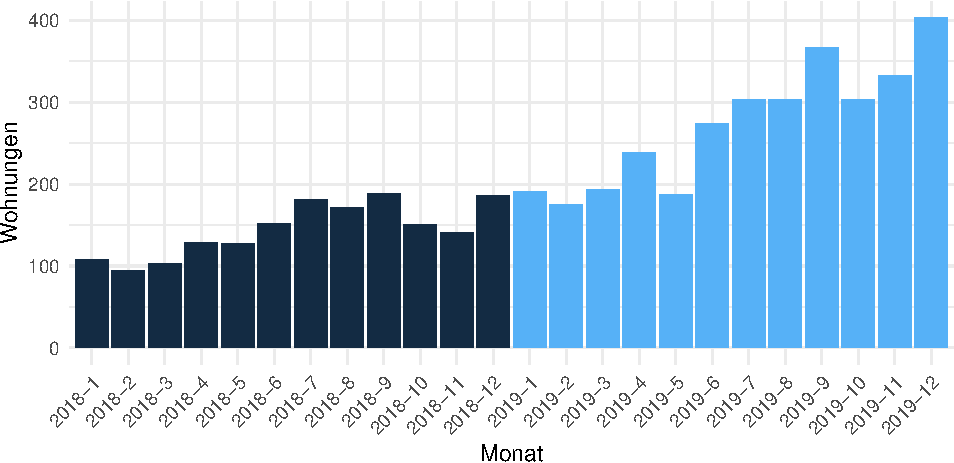
\includegraphics{case_files/figure-latex/unnamed-chunk-1-1.pdf}

\hypertarget{ruxe4umliche-verteilung}{%
\subsubsection{Räumliche Verteilung}\label{ruxe4umliche-verteilung}}

\hypertarget{stadteile}{%
\paragraph{Stadteile}\label{stadteile}}

\begin{columns}

\begin{column}

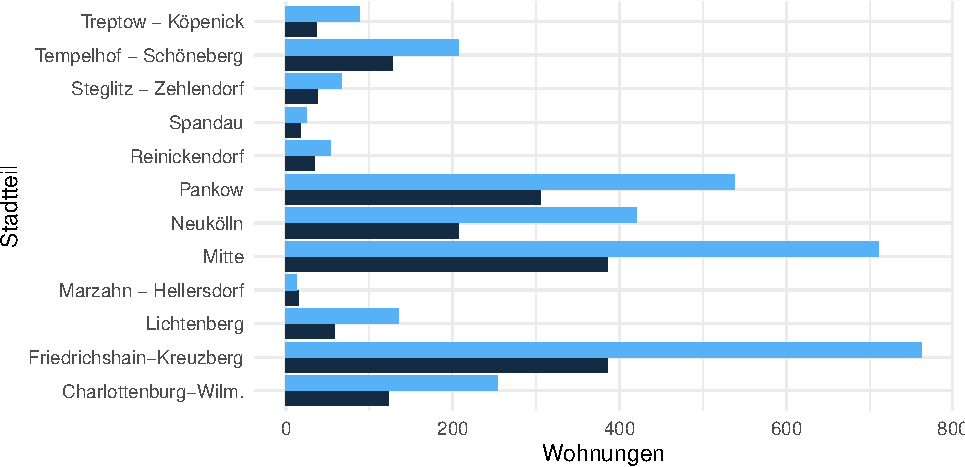
\includegraphics{case_files/figure-latex/unnamed-chunk-2-1.pdf}

\end{column}

\begin{column}

\end{column}

\begin{column}

The figure on the left-hand side shows the \texttt{cars} data.

Lorem ipsum dolor sit amet, consectetur adipiscing elit, sed do eiusmod
tempor incididunt ut labore et dolore magna aliqua. Ut enim ad minim
veniam, quis nostrud exercitation ullamco laboris nisi ut aliquip ex ea
commodo consequat. Duis aute irure dolor in reprehenderit in voluptate
velit esse cillum dolore eu fugiat nulla pariatur.

\end{column}

\end{columns}

\hypertarget{stadteile-uxfcber-die-zeit}{%
\paragraph{Stadteile über die Zeit}\label{stadteile-uxfcber-die-zeit}}

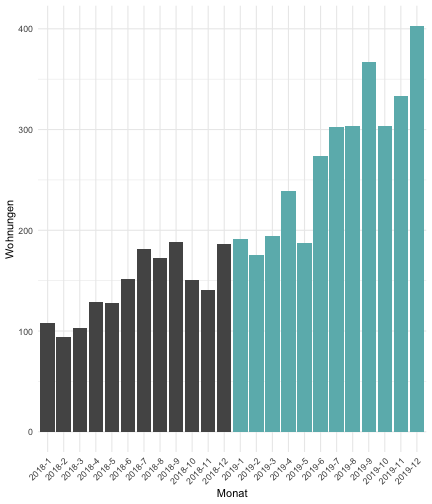
\includegraphics{case_files/figure-latex/unnamed-chunk-3-1.pdf}

\hypertarget{karte}{%
\paragraph{Karte}\label{karte}}

You can also embed plots, for example:

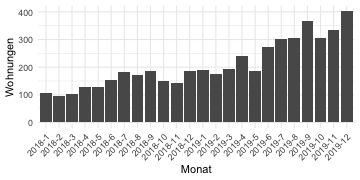
\includegraphics{case_files/figure-latex/unnamed-chunk-4-1.pdf}

\end{document}
